\documentclass[t]{beamer}   

\usepackage{graphicx}

\setbeamertemplate{navigation symbols}{} %remove navigation symbols

% Setting Logo and Template
\usetheme{default}   
\usecolortheme{UCLAsquirrel}
\logo{
\includegraphics[height=0.7cm]{logo_ucla_cw.png}}



% ======================================================================

\begin{document}

\title{Closed-Loop Subspace Identification of a Quadrotor}
\author{Andy Kee}
\institute{University of California, Los Angeles}
\date{September 27, 2013}
\begin{frame}
\titlepage
\end{frame}

% ======================================================================

\begin{frame}\frametitle{Overview}

High-fidelity computer models of dynamical systems continue to play an important role in design and development activities. System identification is the process of developing mathematical models representing system dynamics based on experimentally gathered input-output data.

\

System identification - particularly of Multi-Input Multi-Output (MIMO) systems operating under feedback control (i.e. exhibiting closed-loop dynamics) is of great interest in both academic and commercial domains.

\

It is the goal of this research project to apply subspace system identification techniques to a quadrotor using experimentally gathered closed-loop input and output data.
\end{frame}

% ======================================================================

\begin{frame}\frametitle{The identification problem}
The system identification problem is: \textit{given a set of input-output data, estimate a system model which mimics the dynamics of the physical system as closely as possible.}

\

Traditional system identification techniques develop system models by minimizing prediction error; these techniques are unsurprisingly called Prediction Error Methods (PEMs)

\

While PEMs have seen widespread use in both theoretical and real-world applications,  they experience difficulties when identifying MIMO systems.

\

Subspace identification techniques offer an alternate approach to the identification problem. They have a foundation in linear algebra and are able to identify MIMO systems.  
\end{frame}

% ======================================================================

\begin{frame}\frametitle{Subspace identification}
The subspace identification problem is: \textit{given a set of input-output data, estimate the system matrices (A, B, C, D) up to within a similarity transform.}

\

A generalized subspace identification algorithm is
\begin{itemize}
\item Estimate the extended observable subspace from available input-output data.
\item Extract the system matrices from the extended observable subspace through linear regression.
\end{itemize}

\

Note that specialized filtering and estimation techniques are required to estimate the extended observable subspace in the presence of closed-loop input-output data.
\end{frame}

% ======================================================================

\begin{frame}\frametitle{Quadrotor platform}

\begin{figure}\centering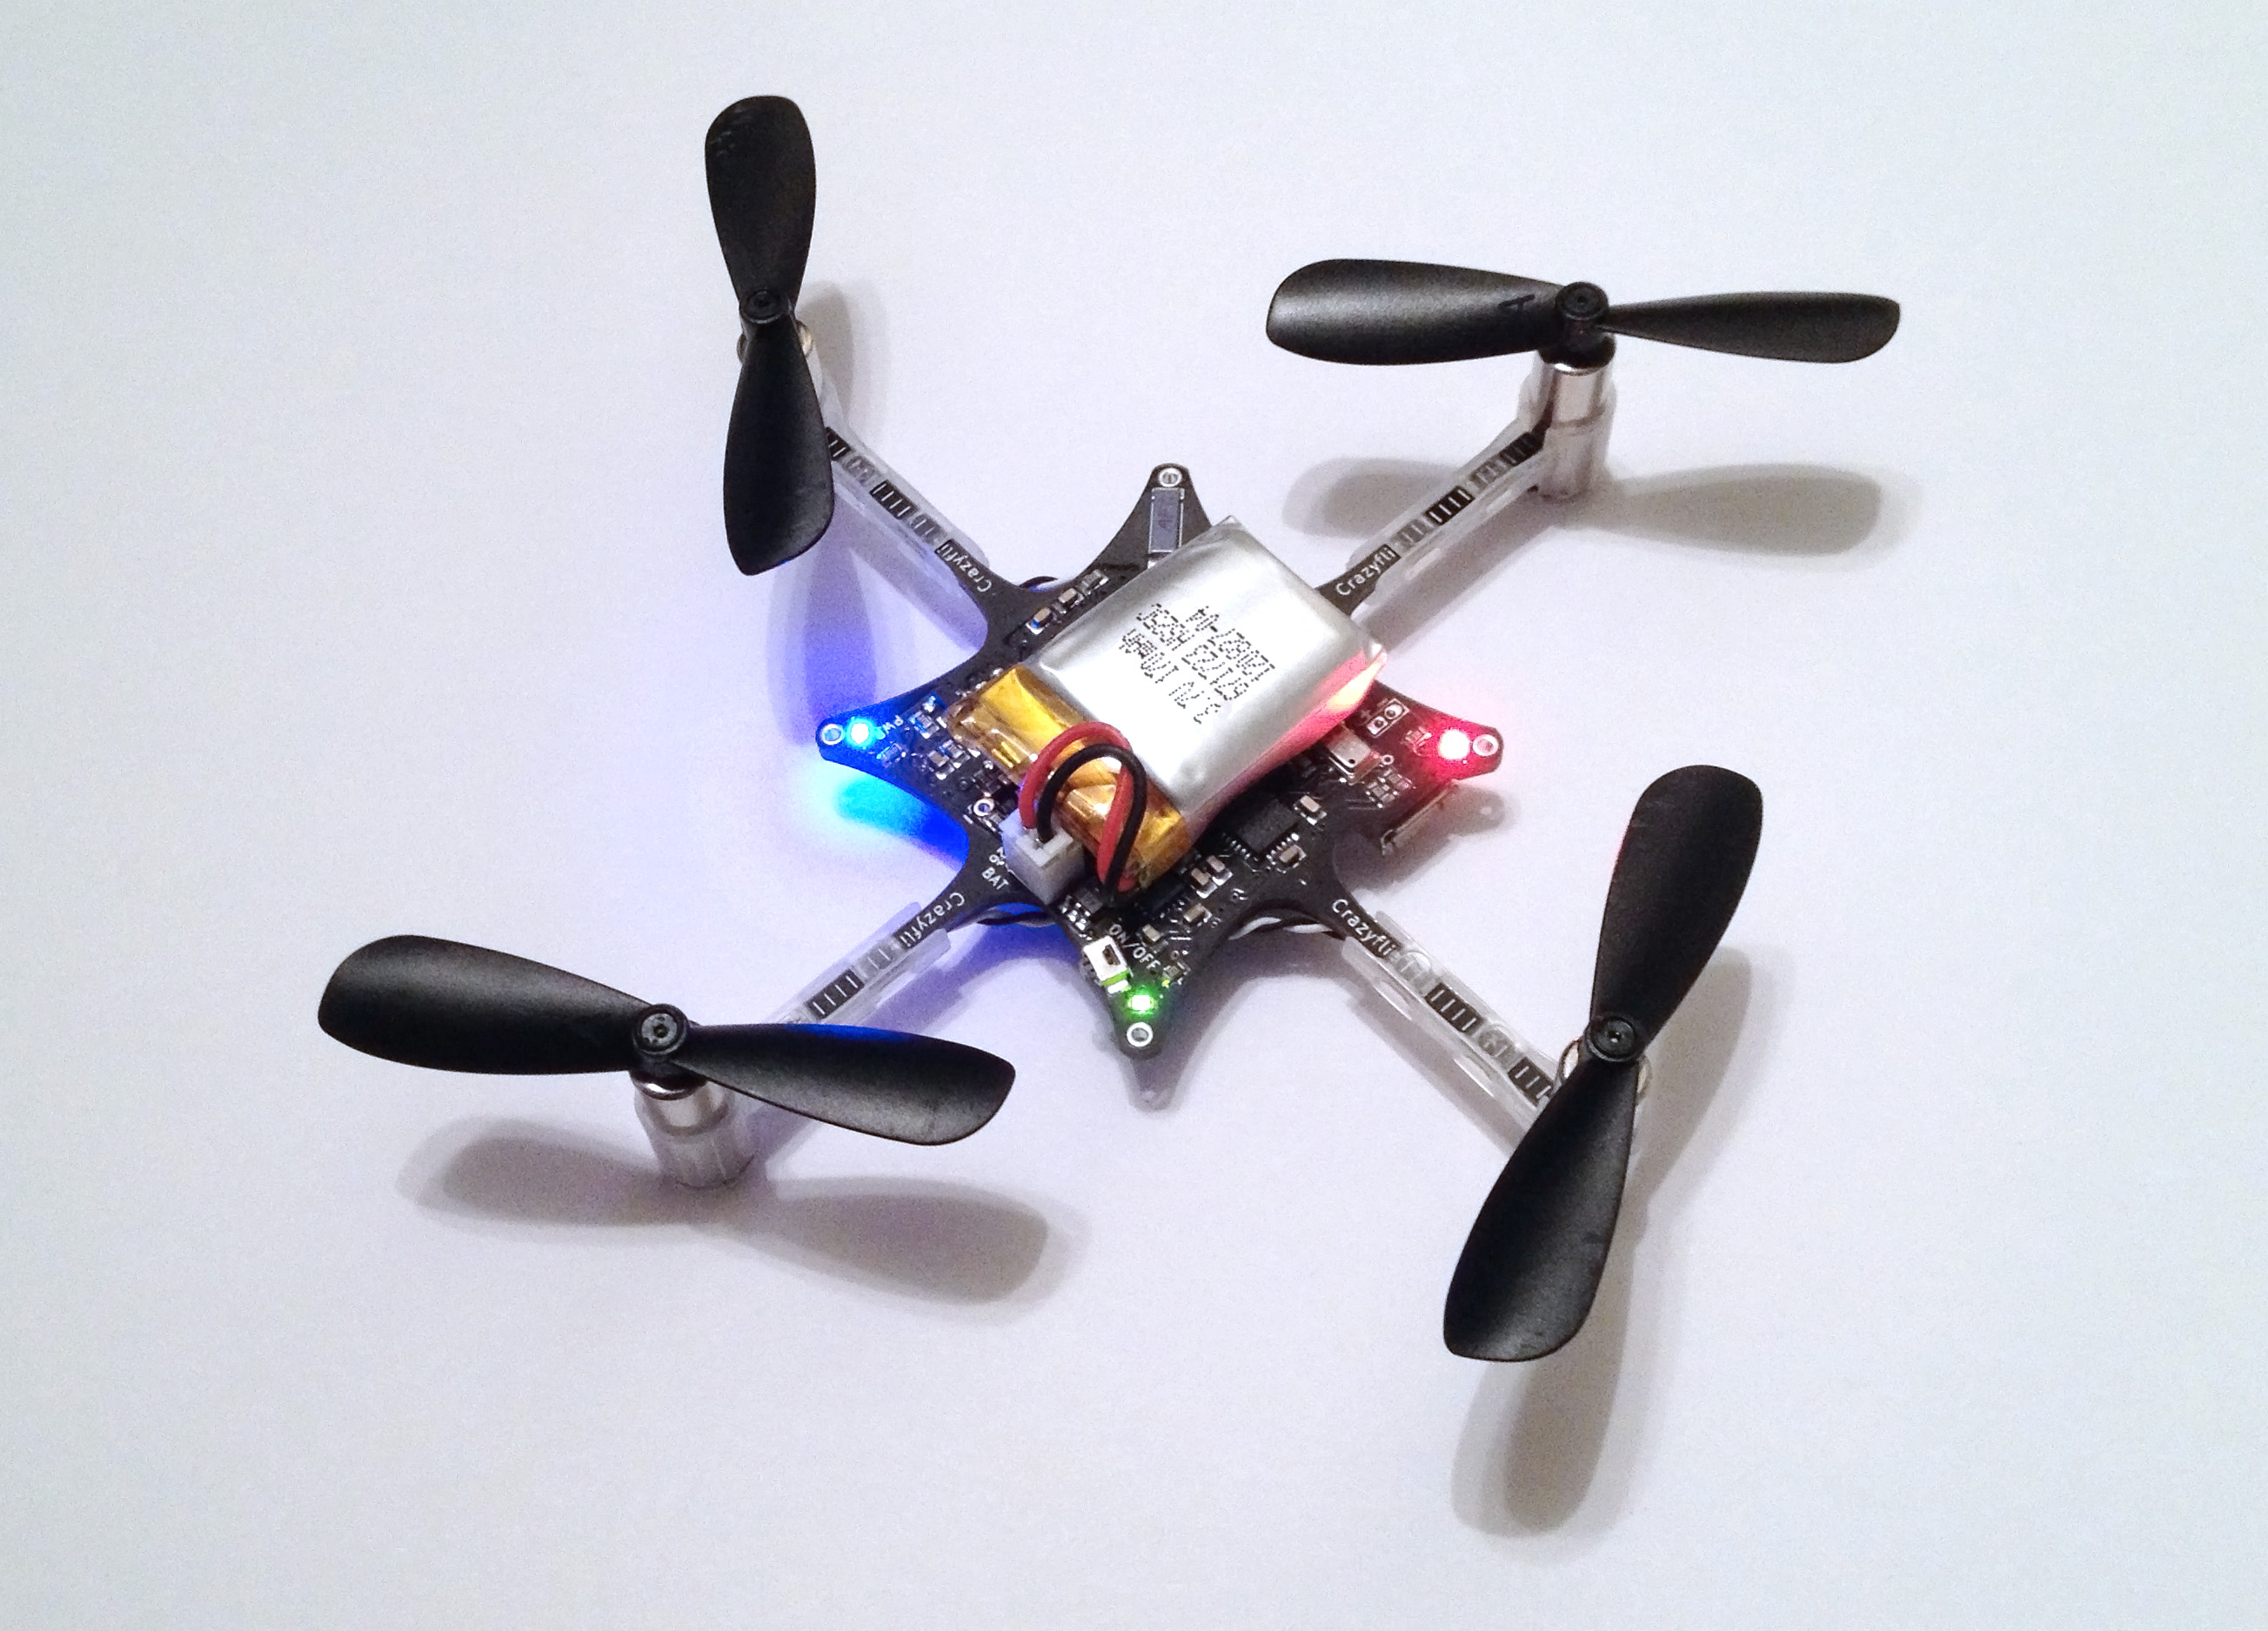
\includegraphics[scale=.07]{crazyflie.jpg}\end{figure}

Bitcraze Crazyflie - an open-source 10DOF quadrotor kit (\$180)

\begin{itemize}
\item 9cm motor to motor, 19g total weight, 7 minute flight time
\item Controlled using any standard USB gamepad connected to a computer running the Crazyflie PC client software
\end{itemize}



\end{frame}

% ======================================================================

\begin{frame}\frametitle{Data collection}

In addition to direct user control, the PC client exposes a Python API making it possible to interact with the quadrotor programmatically.

\

We will perform a series of flight tests by sending the vehicle pseudorandom binary $\phi$, $\theta$, and $\psi$ commands while maintaining constant thrust. The inner-loop control system translates these commands to motor commands.

\

System response is directly measured by the vehicle's onboard sensors - primarily by the three-axis accelerometer and three-axis gyroscope and optionally by the three-axis magnetometer and barometer.

\

The PC client�s logging framework will be used to capture system input-output data.

\end{frame}

% ======================================================================

\begin{frame}\frametitle{PRBS inputs}

\begin{figure}\centering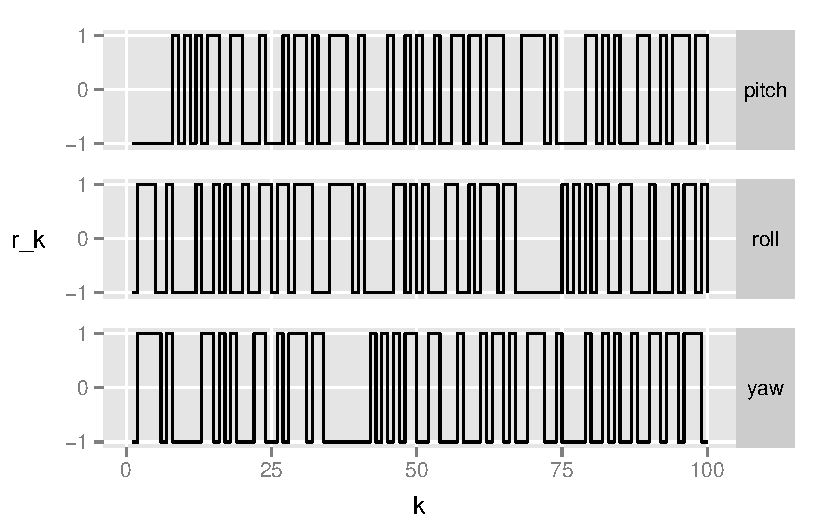
\includegraphics[scale=.7]{prbs_input.pdf}\end{figure}

\end{frame}

% ======================================================================

\begin{frame}\frametitle{Questions?}

\vspace{8em}

\centering
Andy Kee

\texttt{akee@ucla.edu}

\end{frame}

% ======================================================================

\end{document}